\batchmode
\documentclass[twoside]{book}

% Packages required by doxygen
\usepackage{fixltx2e}
\usepackage{calc}
\usepackage{doxygen}
\usepackage[export]{adjustbox} % also loads graphicx
\usepackage{graphicx}
\usepackage[utf8]{inputenc}
\usepackage{makeidx}
\usepackage{multicol}
\usepackage{multirow}
\PassOptionsToPackage{warn}{textcomp}
\usepackage{textcomp}
\usepackage[nointegrals]{wasysym}
\usepackage[table]{xcolor}

% Font selection
\usepackage[T1]{fontenc}
\usepackage[scaled=.90]{helvet}
\usepackage{courier}
\usepackage{amssymb}
\usepackage{sectsty}
\renewcommand{\familydefault}{\sfdefault}
\allsectionsfont{%
  \fontseries{bc}\selectfont%
  \color{darkgray}%
}
\renewcommand{\DoxyLabelFont}{%
  \fontseries{bc}\selectfont%
  \color{darkgray}%
}
\newcommand{\+}{\discretionary{\mbox{\scriptsize$\hookleftarrow$}}{}{}}

% Page & text layout
\usepackage{geometry}
\geometry{%
  a4paper,%
  top=2.5cm,%
  bottom=2.5cm,%
  left=2.5cm,%
  right=2.5cm%
}
\tolerance=750
\hfuzz=15pt
\hbadness=750
\setlength{\emergencystretch}{15pt}
\setlength{\parindent}{0cm}
\setlength{\parskip}{3ex plus 2ex minus 2ex}
\makeatletter
\renewcommand{\paragraph}{%
  \@startsection{paragraph}{4}{0ex}{-1.0ex}{1.0ex}{%
    \normalfont\normalsize\bfseries\SS@parafont%
  }%
}
\renewcommand{\subparagraph}{%
  \@startsection{subparagraph}{5}{0ex}{-1.0ex}{1.0ex}{%
    \normalfont\normalsize\bfseries\SS@subparafont%
  }%
}
\makeatother

% Headers & footers
\usepackage{fancyhdr}
\pagestyle{fancyplain}
\fancyhead[LE]{\fancyplain{}{\bfseries\thepage}}
\fancyhead[CE]{\fancyplain{}{}}
\fancyhead[RE]{\fancyplain{}{\bfseries\leftmark}}
\fancyhead[LO]{\fancyplain{}{\bfseries\rightmark}}
\fancyhead[CO]{\fancyplain{}{}}
\fancyhead[RO]{\fancyplain{}{\bfseries\thepage}}
\fancyfoot[LE]{\fancyplain{}{}}
\fancyfoot[CE]{\fancyplain{}{}}
\fancyfoot[RE]{\fancyplain{}{\bfseries\scriptsize Generated by Doxygen }}
\fancyfoot[LO]{\fancyplain{}{\bfseries\scriptsize Generated by Doxygen }}
\fancyfoot[CO]{\fancyplain{}{}}
\fancyfoot[RO]{\fancyplain{}{}}
\renewcommand{\footrulewidth}{0.4pt}
\renewcommand{\chaptermark}[1]{%
  \markboth{#1}{}%
}
\renewcommand{\sectionmark}[1]{%
  \markright{\thesection\ #1}%
}

% Indices & bibliography
\usepackage{natbib}
\usepackage[titles]{tocloft}
\setcounter{tocdepth}{3}
\setcounter{secnumdepth}{5}
\makeindex

% Hyperlinks (required, but should be loaded last)
\usepackage{ifpdf}
\ifpdf
  \usepackage[pdftex,pagebackref=true]{hyperref}
\else
  \usepackage[ps2pdf,pagebackref=true]{hyperref}
\fi
\hypersetup{%
  colorlinks=true,%
  linkcolor=blue,%
  citecolor=blue,%
  unicode%
}

% Custom commands
\newcommand{\clearemptydoublepage}{%
  \newpage{\pagestyle{empty}\cleardoublepage}%
}

\usepackage{caption}
\captionsetup{labelsep=space,justification=centering,font={bf},singlelinecheck=off,skip=4pt,position=top}

%===== C O N T E N T S =====

\begin{document}

% Titlepage & ToC
\hypersetup{pageanchor=false,
             bookmarksnumbered=true,
             pdfencoding=unicode
            }
\pagenumbering{alph}
\begin{titlepage}
\vspace*{7cm}
\begin{center}%
{\Large Assignment 1 }\\
\vspace*{1cm}
{\large Generated by Doxygen 1.8.13}\\
\end{center}
\end{titlepage}
\clearemptydoublepage
\pagenumbering{roman}
\tableofcontents
\clearemptydoublepage
\pagenumbering{arabic}
\hypersetup{pageanchor=true}

%--- Begin generated contents ---
\chapter{Hierarchical Index}
\section{Class Hierarchy}
This inheritance list is sorted roughly, but not completely, alphabetically\+:\begin{DoxyCompactList}
\item \contentsline{section}{complex\+\_\+adt.\+ComplexT}{\pageref{classcomplex__adt_1_1_complex_t}}{}
\item \contentsline{section}{triangle\+\_\+adt.\+TriangleT}{\pageref{classtriangle__adt_1_1_triangle_t}}{}
\item Enum\begin{DoxyCompactList}
\item \contentsline{section}{triangle\+\_\+adt.\+Tri\+Type}{\pageref{classtriangle__adt_1_1_tri_type}}{}
\end{DoxyCompactList}
\end{DoxyCompactList}

\chapter{Class Index}
\section{Class List}
Here are the classes, structs, unions and interfaces with brief descriptions\+:\begin{DoxyCompactList}
\item\contentsline{section}{\hyperlink{classcomplex__adt_1_1_complex_t}{complex\+\_\+adt.\+ComplexT} }{\pageref{classcomplex__adt_1_1_complex_t}}{}
\item\contentsline{section}{\hyperlink{classtriangle__adt_1_1_triangle_t}{triangle\+\_\+adt.\+TriangleT} }{\pageref{classtriangle__adt_1_1_triangle_t}}{}
\item\contentsline{section}{\hyperlink{classtriangle__adt_1_1_tri_type}{triangle\+\_\+adt.\+Tri\+Type} \\*An enumerated data type that represents different types of triangles }{\pageref{classtriangle__adt_1_1_tri_type}}{}
\end{DoxyCompactList}

\chapter{File Index}
\section{File List}
Here is a list of all documented files with brief descriptions\+:\begin{DoxyCompactList}
\item\contentsline{section}{src/\hyperlink{complex__adt_8py}{complex\+\_\+adt.\+py} \\*Provides methods for performing calculations on complex numbers }{\pageref{complex__adt_8py}}{}
\item\contentsline{section}{src/\hyperlink{triangle__adt_8py}{triangle\+\_\+adt.\+py} \\*Provides methods for performing calculations on complex numbers }{\pageref{triangle__adt_8py}}{}
\end{DoxyCompactList}

\chapter{Class Documentation}
\hypertarget{classcomplex__adt_1_1_complex_t}{}\section{complex\+\_\+adt.\+ComplexT Class Reference}
\label{classcomplex__adt_1_1_complex_t}\index{complex\+\_\+adt.\+ComplexT@{complex\+\_\+adt.\+ComplexT}}
\subsection*{Public Member Functions}
\begin{DoxyCompactItemize}
\item 
def \hyperlink{classcomplex__adt_1_1_complex_t_a548b6a454baa3e00a51bde429b5f0eee}{\+\_\+\+\_\+init\+\_\+\+\_\+}
\begin{DoxyCompactList}\small\item\em \hyperlink{classcomplex__adt_1_1_complex_t}{ComplexT} constructor. \end{DoxyCompactList}\end{DoxyCompactItemize}
\subsection*{Public Attributes}
\begin{DoxyCompactItemize}
\item 
\mbox{\Hypertarget{classcomplex__adt_1_1_complex_t_a1aad64f976e595cfcd696df5d0409962}\label{classcomplex__adt_1_1_complex_t_a1aad64f976e595cfcd696df5d0409962}} 
{\bfseries x}
\item 
\mbox{\Hypertarget{classcomplex__adt_1_1_complex_t_a31481d8250df9e06d34687fe719bbd63}\label{classcomplex__adt_1_1_complex_t_a31481d8250df9e06d34687fe719bbd63}} 
{\bfseries y}
\end{DoxyCompactItemize}


\subsection{Constructor \& Destructor Documentation}
\mbox{\Hypertarget{classcomplex__adt_1_1_complex_t_a548b6a454baa3e00a51bde429b5f0eee}\label{classcomplex__adt_1_1_complex_t_a548b6a454baa3e00a51bde429b5f0eee}} 
\index{complex\+\_\+adt\+::\+ComplexT@{complex\+\_\+adt\+::\+ComplexT}!\+\_\+\+\_\+init\+\_\+\+\_\+@{\+\_\+\+\_\+init\+\_\+\+\_\+}}
\index{\+\_\+\+\_\+init\+\_\+\+\_\+@{\+\_\+\+\_\+init\+\_\+\+\_\+}!complex\+\_\+adt\+::\+ComplexT@{complex\+\_\+adt\+::\+ComplexT}}
\subsubsection{\texorpdfstring{\+\_\+\+\_\+init\+\_\+\+\_\+()}{\_\_init\_\_()}}
{\footnotesize\ttfamily def complex\+\_\+adt.\+Complex\+T.\+\_\+\+\_\+init\+\_\+\+\_\+ (\begin{DoxyParamCaption}\item[{}]{self,  }\item[{}]{x }\end{DoxyParamCaption})}



\hyperlink{classcomplex__adt_1_1_complex_t}{ComplexT} constructor. 

Initializes a \hyperlink{classcomplex__adt_1_1_complex_t}{ComplexT} object with real part and an imaginary part. It also rounds the value of both real and imaginary parts upto five decimal points. Assumption is made that the both inputs are of floating point type. 
\begin{DoxyParams}{Parameters}
{\em x} & The real part of the \hyperlink{classcomplex__adt_1_1_complex_t}{ComplexT} object. \\
\hline
{\em y} & The imaginary part of the \hyperlink{classcomplex__adt_1_1_complex_t}{ComplexT} object. \\
\hline
\end{DoxyParams}


The documentation for this class was generated from the following file\+:\begin{DoxyCompactItemize}
\item 
src/\hyperlink{complex__adt_8py}{complex\+\_\+adt.\+py}\end{DoxyCompactItemize}

\hypertarget{classtriangle__adt_1_1_triangle_t}{}\section{triangle\+\_\+adt.\+TriangleT Class Reference}
\label{classtriangle__adt_1_1_triangle_t}\index{triangle\+\_\+adt.\+TriangleT@{triangle\+\_\+adt.\+TriangleT}}
\subsection*{Public Member Functions}
\begin{DoxyCompactItemize}
\item 
def \hyperlink{classtriangle__adt_1_1_triangle_t_a9837232c07fac634ba677a44fc3fee96}{\+\_\+\+\_\+init\+\_\+\+\_\+}
\begin{DoxyCompactList}\small\item\em \hyperlink{classtriangle__adt_1_1_triangle_t}{TriangleT} constructor. \end{DoxyCompactList}\item 
def \hyperlink{classtriangle__adt_1_1_triangle_t_a598e20e41e186231c9103a6249f9eeb6}{get\+\_\+sides} (self)
\begin{DoxyCompactList}\small\item\em Gets all the lenght of sides of a triangle. \end{DoxyCompactList}\item 
def \hyperlink{classtriangle__adt_1_1_triangle_t_aa7615cb08eac693134dd4022d984c8ec}{equal} (self, t)
\begin{DoxyCompactList}\small\item\em Checks if two \hyperlink{classtriangle__adt_1_1_triangle_t}{TriangleT} objects are equal or not. \end{DoxyCompactList}\item 
def \hyperlink{classtriangle__adt_1_1_triangle_t_aeb7d763a098e7d8d23b78c69d375154c}{perim} (self)
\begin{DoxyCompactList}\small\item\em Calculates the perimeter of a \hyperlink{classtriangle__adt_1_1_triangle_t}{TriangleT} object by adding all the lenghts of sides. \end{DoxyCompactList}\item 
def \hyperlink{classtriangle__adt_1_1_triangle_t_a61a982c7a989dc80764cbf7c79ec048b}{area} (self)
\begin{DoxyCompactList}\small\item\em Calculates the area of a \hyperlink{classtriangle__adt_1_1_triangle_t}{TriangleT} object by using herons formula. \end{DoxyCompactList}\item 
def \hyperlink{classtriangle__adt_1_1_triangle_t_a2edd73d4eb4aedae932161c1befb5c63}{is\+\_\+valid} (self)
\begin{DoxyCompactList}\small\item\em Checks if \hyperlink{classtriangle__adt_1_1_triangle_t}{TriangleT} object is valid. \end{DoxyCompactList}\item 
def \hyperlink{classtriangle__adt_1_1_triangle_t_af33c895ca41f21cfc6441af8192a7998}{tri\+\_\+type} (self)
\begin{DoxyCompactList}\small\item\em Checks what type of Triangle the \hyperlink{classtriangle__adt_1_1_triangle_t}{TriangleT} object is. \end{DoxyCompactList}\end{DoxyCompactItemize}
\subsection*{Public Attributes}
\begin{DoxyCompactItemize}
\item 
\mbox{\Hypertarget{classtriangle__adt_1_1_triangle_t_a678fbcb3fdd76f4787bc3d8a437fc84f}\label{classtriangle__adt_1_1_triangle_t_a678fbcb3fdd76f4787bc3d8a437fc84f}} 
{\bfseries s}
\end{DoxyCompactItemize}


\subsection{Constructor \& Destructor Documentation}
\mbox{\Hypertarget{classtriangle__adt_1_1_triangle_t_a9837232c07fac634ba677a44fc3fee96}\label{classtriangle__adt_1_1_triangle_t_a9837232c07fac634ba677a44fc3fee96}} 
\index{triangle\+\_\+adt\+::\+TriangleT@{triangle\+\_\+adt\+::\+TriangleT}!\+\_\+\+\_\+init\+\_\+\+\_\+@{\+\_\+\+\_\+init\+\_\+\+\_\+}}
\index{\+\_\+\+\_\+init\+\_\+\+\_\+@{\+\_\+\+\_\+init\+\_\+\+\_\+}!triangle\+\_\+adt\+::\+TriangleT@{triangle\+\_\+adt\+::\+TriangleT}}
\subsubsection{\texorpdfstring{\+\_\+\+\_\+init\+\_\+\+\_\+()}{\_\_init\_\_()}}
{\footnotesize\ttfamily def triangle\+\_\+adt.\+Triangle\+T.\+\_\+\+\_\+init\+\_\+\+\_\+ (\begin{DoxyParamCaption}\item[{}]{self,  }\item[{}]{a }\end{DoxyParamCaption})}



\hyperlink{classtriangle__adt_1_1_triangle_t}{TriangleT} constructor. 

Initializes a \hyperlink{classtriangle__adt_1_1_triangle_t}{TriangleT} object by taking three sides as input. Assumption is made that all the inputs are of integer types. 
\begin{DoxyParams}{Parameters}
{\em a} & The length of first side of triangle. \\
\hline
{\em b} & The length of second side of triangle. \\
\hline
{\em c} & The length of third side of triangle. \\
\hline
\end{DoxyParams}


\subsection{Member Function Documentation}
\mbox{\Hypertarget{classtriangle__adt_1_1_triangle_t_a61a982c7a989dc80764cbf7c79ec048b}\label{classtriangle__adt_1_1_triangle_t_a61a982c7a989dc80764cbf7c79ec048b}} 
\index{triangle\+\_\+adt\+::\+TriangleT@{triangle\+\_\+adt\+::\+TriangleT}!area@{area}}
\index{area@{area}!triangle\+\_\+adt\+::\+TriangleT@{triangle\+\_\+adt\+::\+TriangleT}}
\subsubsection{\texorpdfstring{area()}{area()}}
{\footnotesize\ttfamily def triangle\+\_\+adt.\+Triangle\+T.\+area (\begin{DoxyParamCaption}\item[{}]{self }\end{DoxyParamCaption})}



Calculates the area of a \hyperlink{classtriangle__adt_1_1_triangle_t}{TriangleT} object by using herons formula. 


\begin{DoxyExceptions}{Exceptions}
{\em Triangle\+Not\+Valid} & Throws Triangle\+Not\+Valid if \hyperlink{classtriangle__adt_1_1_triangle_t}{TriangleT} object is not valid. \\
\hline
\end{DoxyExceptions}
\begin{DoxyReturn}{Returns}
Area of \hyperlink{classtriangle__adt_1_1_triangle_t}{TriangleT} object. 
\end{DoxyReturn}
\mbox{\Hypertarget{classtriangle__adt_1_1_triangle_t_aa7615cb08eac693134dd4022d984c8ec}\label{classtriangle__adt_1_1_triangle_t_aa7615cb08eac693134dd4022d984c8ec}} 
\index{triangle\+\_\+adt\+::\+TriangleT@{triangle\+\_\+adt\+::\+TriangleT}!equal@{equal}}
\index{equal@{equal}!triangle\+\_\+adt\+::\+TriangleT@{triangle\+\_\+adt\+::\+TriangleT}}
\subsubsection{\texorpdfstring{equal()}{equal()}}
{\footnotesize\ttfamily def triangle\+\_\+adt.\+Triangle\+T.\+equal (\begin{DoxyParamCaption}\item[{}]{self,  }\item[{}]{t }\end{DoxyParamCaption})}



Checks if two \hyperlink{classtriangle__adt_1_1_triangle_t}{TriangleT} objects are equal or not. 

param t \hyperlink{classtriangle__adt_1_1_triangle_t}{TriangleT} object evaluated for equality. 
\begin{DoxyExceptions}{Exceptions}
{\em Triangle\+Not\+Valid} & Throws Triangle\+Not\+Valid if \hyperlink{classtriangle__adt_1_1_triangle_t}{TriangleT} object is not valid. \\
\hline
\end{DoxyExceptions}
\begin{DoxyReturn}{Returns}
Returns true if the \hyperlink{classtriangle__adt_1_1_triangle_t}{TriangleT} object is equal with the given \hyperlink{classtriangle__adt_1_1_triangle_t}{TriangleT} object; false if not 
\end{DoxyReturn}
\mbox{\Hypertarget{classtriangle__adt_1_1_triangle_t_a598e20e41e186231c9103a6249f9eeb6}\label{classtriangle__adt_1_1_triangle_t_a598e20e41e186231c9103a6249f9eeb6}} 
\index{triangle\+\_\+adt\+::\+TriangleT@{triangle\+\_\+adt\+::\+TriangleT}!get\+\_\+sides@{get\+\_\+sides}}
\index{get\+\_\+sides@{get\+\_\+sides}!triangle\+\_\+adt\+::\+TriangleT@{triangle\+\_\+adt\+::\+TriangleT}}
\subsubsection{\texorpdfstring{get\+\_\+sides()}{get\_sides()}}
{\footnotesize\ttfamily def triangle\+\_\+adt.\+Triangle\+T.\+get\+\_\+sides (\begin{DoxyParamCaption}\item[{}]{self }\end{DoxyParamCaption})}



Gets all the lenght of sides of a triangle. 

\begin{DoxyReturn}{Returns}
A tuple of lengths of sides in a sorted order. 
\end{DoxyReturn}
\mbox{\Hypertarget{classtriangle__adt_1_1_triangle_t_a2edd73d4eb4aedae932161c1befb5c63}\label{classtriangle__adt_1_1_triangle_t_a2edd73d4eb4aedae932161c1befb5c63}} 
\index{triangle\+\_\+adt\+::\+TriangleT@{triangle\+\_\+adt\+::\+TriangleT}!is\+\_\+valid@{is\+\_\+valid}}
\index{is\+\_\+valid@{is\+\_\+valid}!triangle\+\_\+adt\+::\+TriangleT@{triangle\+\_\+adt\+::\+TriangleT}}
\subsubsection{\texorpdfstring{is\+\_\+valid()}{is\_valid()}}
{\footnotesize\ttfamily def triangle\+\_\+adt.\+Triangle\+T.\+is\+\_\+valid (\begin{DoxyParamCaption}\item[{}]{self }\end{DoxyParamCaption})}



Checks if \hyperlink{classtriangle__adt_1_1_triangle_t}{TriangleT} object is valid. 

Checks validity of \hyperlink{classtriangle__adt_1_1_triangle_t}{TriangleT} by checking if the sum of any two sides would be less or equal to the third side. \begin{DoxyReturn}{Returns}
Returns true if the \hyperlink{classtriangle__adt_1_1_triangle_t}{TriangleT} object is valid; false if not. 
\end{DoxyReturn}
\mbox{\Hypertarget{classtriangle__adt_1_1_triangle_t_aeb7d763a098e7d8d23b78c69d375154c}\label{classtriangle__adt_1_1_triangle_t_aeb7d763a098e7d8d23b78c69d375154c}} 
\index{triangle\+\_\+adt\+::\+TriangleT@{triangle\+\_\+adt\+::\+TriangleT}!perim@{perim}}
\index{perim@{perim}!triangle\+\_\+adt\+::\+TriangleT@{triangle\+\_\+adt\+::\+TriangleT}}
\subsubsection{\texorpdfstring{perim()}{perim()}}
{\footnotesize\ttfamily def triangle\+\_\+adt.\+Triangle\+T.\+perim (\begin{DoxyParamCaption}\item[{}]{self }\end{DoxyParamCaption})}



Calculates the perimeter of a \hyperlink{classtriangle__adt_1_1_triangle_t}{TriangleT} object by adding all the lenghts of sides. 


\begin{DoxyExceptions}{Exceptions}
{\em Triangle\+Not\+Valid} & Throws Triangle\+Not\+Valid if \hyperlink{classtriangle__adt_1_1_triangle_t}{TriangleT} object is not valid. \\
\hline
\end{DoxyExceptions}
\begin{DoxyReturn}{Returns}
Sum of all lengths of sides. 
\end{DoxyReturn}
\mbox{\Hypertarget{classtriangle__adt_1_1_triangle_t_af33c895ca41f21cfc6441af8192a7998}\label{classtriangle__adt_1_1_triangle_t_af33c895ca41f21cfc6441af8192a7998}} 
\index{triangle\+\_\+adt\+::\+TriangleT@{triangle\+\_\+adt\+::\+TriangleT}!tri\+\_\+type@{tri\+\_\+type}}
\index{tri\+\_\+type@{tri\+\_\+type}!triangle\+\_\+adt\+::\+TriangleT@{triangle\+\_\+adt\+::\+TriangleT}}
\subsubsection{\texorpdfstring{tri\+\_\+type()}{tri\_type()}}
{\footnotesize\ttfamily def triangle\+\_\+adt.\+Triangle\+T.\+tri\+\_\+type (\begin{DoxyParamCaption}\item[{}]{self }\end{DoxyParamCaption})}



Checks what type of Triangle the \hyperlink{classtriangle__adt_1_1_triangle_t}{TriangleT} object is. 


\begin{DoxyExceptions}{Exceptions}
{\em Triangle\+Not\+Valid} & Throws Triangle\+Not\+Valid if \hyperlink{classtriangle__adt_1_1_triangle_t}{TriangleT} object is not valid.\\
\hline
\end{DoxyExceptions}
The triangle type is checked by applying different formulas for which Right,Scalene,Isosceles and Equilateral will hold true. Right Angle Triangle type objects have the highest precedency. \begin{DoxyReturn}{Returns}
The type of \hyperlink{classtriangle__adt_1_1_triangle_t}{TriangleT} object. 
\end{DoxyReturn}


The documentation for this class was generated from the following file\+:\begin{DoxyCompactItemize}
\item 
src/\hyperlink{triangle__adt_8py}{triangle\+\_\+adt.\+py}\end{DoxyCompactItemize}

\hypertarget{classtriangle__adt_1_1_tri_type}{}\section{triangle\+\_\+adt.\+Tri\+Type Class Reference}
\label{classtriangle__adt_1_1_tri_type}\index{triangle\+\_\+adt.\+Tri\+Type@{triangle\+\_\+adt.\+Tri\+Type}}


An enumerated data type that represents different types of triangles.  


Inheritance diagram for triangle\+\_\+adt.\+Tri\+Type\+:\begin{figure}[H]
\begin{center}
\leavevmode
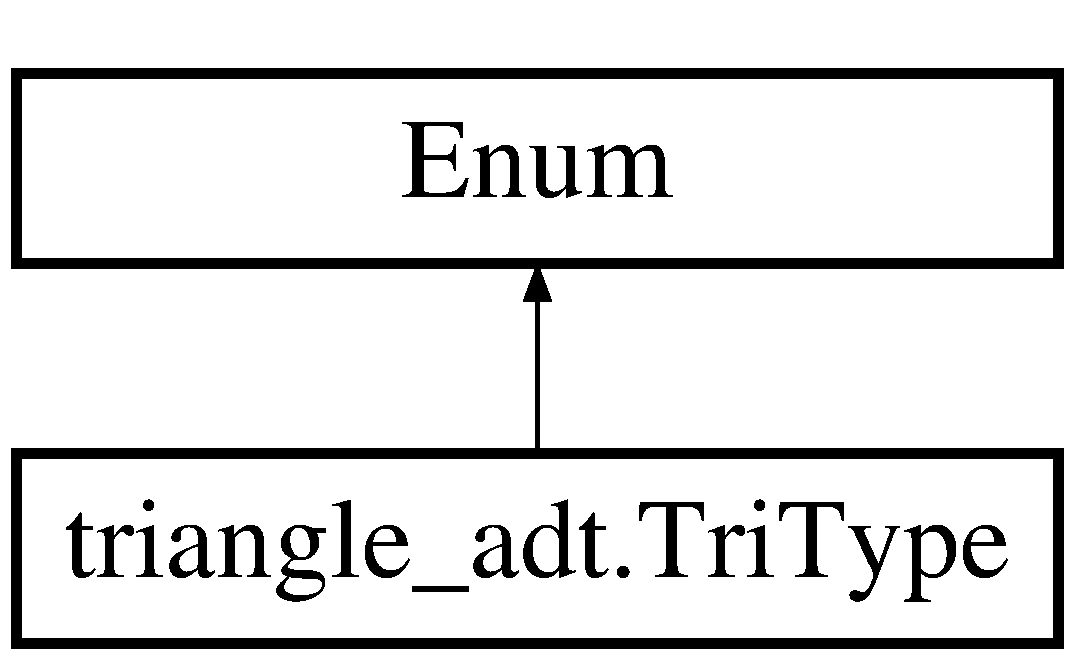
\includegraphics[height=2.000000cm]{classtriangle__adt_1_1_tri_type}
\end{center}
\end{figure}
\subsection*{Static Public Attributes}
\begin{DoxyCompactItemize}
\item 
\mbox{\Hypertarget{classtriangle__adt_1_1_tri_type_a0eb98494388109343f9f159cc19db806}\label{classtriangle__adt_1_1_tri_type_a0eb98494388109343f9f159cc19db806}} 
int {\bfseries equilat} = 1
\item 
\mbox{\Hypertarget{classtriangle__adt_1_1_tri_type_a4365f5f84ae196c8a683a2410047d151}\label{classtriangle__adt_1_1_tri_type_a4365f5f84ae196c8a683a2410047d151}} 
int {\bfseries isosceles} = 2
\item 
\mbox{\Hypertarget{classtriangle__adt_1_1_tri_type_a02b27c62da67a95c7721c164b2671298}\label{classtriangle__adt_1_1_tri_type_a02b27c62da67a95c7721c164b2671298}} 
int {\bfseries scalene} = 3
\item 
\mbox{\Hypertarget{classtriangle__adt_1_1_tri_type_a194e9713b488d32aac5554803dc2ddba}\label{classtriangle__adt_1_1_tri_type_a194e9713b488d32aac5554803dc2ddba}} 
int {\bfseries right} = 4
\end{DoxyCompactItemize}


\subsection{Detailed Description}
An enumerated data type that represents different types of triangles. 



The documentation for this class was generated from the following file\+:\begin{DoxyCompactItemize}
\item 
src/\hyperlink{triangle__adt_8py}{triangle\+\_\+adt.\+py}\end{DoxyCompactItemize}

\chapter{File Documentation}
\hypertarget{complex__adt_8py}{}\section{src/complex\+\_\+adt.py File Reference}
\label{complex__adt_8py}\index{src/complex\+\_\+adt.\+py@{src/complex\+\_\+adt.\+py}}


Provides methods for performing calculations on complex numbers.  


\subsection*{Classes}
\begin{DoxyCompactItemize}
\item 
class \hyperlink{classcomplex__adt_1_1_complex_t}{complex\+\_\+adt.\+ComplexT}
\end{DoxyCompactItemize}
\subsection*{Functions}
\begin{DoxyCompactItemize}
\item 
def \hyperlink{complex__adt_8py_a2e278aa3958b187d63c6358a3b445dac}{complex\+\_\+adt.\+real} (self)
\begin{DoxyCompactList}\small\item\em Gets the real part of the \hyperlink{classcomplex__adt_1_1_complex_t}{ComplexT} object. \end{DoxyCompactList}\item 
def \hyperlink{complex__adt_8py_ac4caba6b40cace9a6757f4942bed7073}{complex\+\_\+adt.\+imag} (self)
\begin{DoxyCompactList}\small\item\em imag Gets the imaginary part of the \hyperlink{classcomplex__adt_1_1_complex_t}{ComplexT} object. \end{DoxyCompactList}\item 
def \hyperlink{complex__adt_8py_a380fce54280bbd60eb1d88ea135461f4}{complex\+\_\+adt.\+get\+\_\+r} (self)
\begin{DoxyCompactList}\small\item\em get\+\_\+r Calculates the modulus of the \hyperlink{classcomplex__adt_1_1_complex_t}{ComplexT} object. \end{DoxyCompactList}\item 
def \hyperlink{complex__adt_8py_a54c73b9611d25b015f7665090706d2b2}{complex\+\_\+adt.\+get\+\_\+phi} (self)
\begin{DoxyCompactList}\small\item\em Calculates the phase(argument) between the \hyperlink{classcomplex__adt_1_1_complex_t}{ComplexT} object. \end{DoxyCompactList}\item 
def \hyperlink{complex__adt_8py_a5424e66eac1da858be5ecd6e4008fc9f}{complex\+\_\+adt.\+equal} (self, c)
\begin{DoxyCompactList}\small\item\em Check if the two complex numbers are equal or not. \end{DoxyCompactList}\item 
def \hyperlink{complex__adt_8py_aa3db7ee93ebc8b350db389b1bd544135}{complex\+\_\+adt.\+conj} (self)
\begin{DoxyCompactList}\small\item\em Does the negation of the imaginary part. \end{DoxyCompactList}\item 
def \hyperlink{complex__adt_8py_a3367e3cac848f6a7327cf8f2dc423947}{complex\+\_\+adt.\+add} (self, a)
\begin{DoxyCompactList}\small\item\em Adds the two \hyperlink{classcomplex__adt_1_1_complex_t}{ComplexT} objects. \end{DoxyCompactList}\item 
def \hyperlink{complex__adt_8py_aa4c911dafbd349f35afb3fcc7f9ddc30}{complex\+\_\+adt.\+sub} (self, a)
\begin{DoxyCompactList}\small\item\em Subtracts the two \hyperlink{classcomplex__adt_1_1_complex_t}{ComplexT} objects. \end{DoxyCompactList}\item 
def \hyperlink{complex__adt_8py_aee6948250c74aa21fc689d5b7b85d818}{complex\+\_\+adt.\+mult} (self, a)
\begin{DoxyCompactList}\small\item\em Multiplies two \hyperlink{classcomplex__adt_1_1_complex_t}{ComplexT} objects. \end{DoxyCompactList}\item 
def \hyperlink{complex__adt_8py_a1e25fca2604ff729f81107fcc3ff9099}{complex\+\_\+adt.\+recip} (self)
\begin{DoxyCompactList}\small\item\em Divides one by the \hyperlink{classcomplex__adt_1_1_complex_t}{ComplexT} object. \end{DoxyCompactList}\item 
def \hyperlink{complex__adt_8py_af5b4032d0854249f575b49011d6a33b4}{complex\+\_\+adt.\+div} (self, a)
\begin{DoxyCompactList}\small\item\em Divides the two \hyperlink{classcomplex__adt_1_1_complex_t}{ComplexT} objects. \end{DoxyCompactList}\item 
def \hyperlink{complex__adt_8py_aef2a4c489ff133a870a1405b8910e3da}{complex\+\_\+adt.\+sqrt} (self)
\begin{DoxyCompactList}\small\item\em Finds the square root of the \hyperlink{classcomplex__adt_1_1_complex_t}{ComplexT} object. \end{DoxyCompactList}\end{DoxyCompactItemize}


\subsection{Detailed Description}
Provides methods for performing calculations on complex numbers. 

\begin{DoxyAuthor}{Author}
Harkanwar Singh Waraich 
\end{DoxyAuthor}
\begin{DoxyDate}{Date}
01/14/2021 
\end{DoxyDate}


\subsection{Function Documentation}
\mbox{\Hypertarget{complex__adt_8py_file_a3367e3cac848f6a7327cf8f2dc423947}\label{complex__adt_8py_file_a3367e3cac848f6a7327cf8f2dc423947}} 
\index{complex\+\_\+adt.\+py@{complex\+\_\+adt.\+py}!add@{add}}
\index{add@{add}!complex\+\_\+adt.\+py@{complex\+\_\+adt.\+py}}
\subsubsection{\texorpdfstring{add()}{add()}}
{\footnotesize\ttfamily def complex\+\_\+adt.\+add (\begin{DoxyParamCaption}\item[{}]{self,  }\item[{}]{a }\end{DoxyParamCaption})}



Adds the two ComplexT objects. 


\begin{DoxyParams}{Parameters}
{\em a} & ComplexT object to be added. \\
\hline
\end{DoxyParams}
\begin{DoxyReturn}{Returns}
Addition of two ComplexT objects. 
\end{DoxyReturn}
\mbox{\Hypertarget{complex__adt_8py_file_aa3db7ee93ebc8b350db389b1bd544135}\label{complex__adt_8py_file_aa3db7ee93ebc8b350db389b1bd544135}} 
\index{complex\+\_\+adt.\+py@{complex\+\_\+adt.\+py}!conj@{conj}}
\index{conj@{conj}!complex\+\_\+adt.\+py@{complex\+\_\+adt.\+py}}
\subsubsection{\texorpdfstring{conj()}{conj()}}
{\footnotesize\ttfamily def complex\+\_\+adt.\+conj (\begin{DoxyParamCaption}\item[{}]{self }\end{DoxyParamCaption})}



Does the negation of the imaginary part. 

\begin{DoxyReturn}{Returns}
The same object but with the negation of the imaginary part 
\end{DoxyReturn}
\mbox{\Hypertarget{complex__adt_8py_file_af5b4032d0854249f575b49011d6a33b4}\label{complex__adt_8py_file_af5b4032d0854249f575b49011d6a33b4}} 
\index{complex\+\_\+adt.\+py@{complex\+\_\+adt.\+py}!div@{div}}
\index{div@{div}!complex\+\_\+adt.\+py@{complex\+\_\+adt.\+py}}
\subsubsection{\texorpdfstring{div()}{div()}}
{\footnotesize\ttfamily def complex\+\_\+adt.\+div (\begin{DoxyParamCaption}\item[{}]{self,  }\item[{}]{a }\end{DoxyParamCaption})}



Divides the two ComplexT objects. 


\begin{DoxyExceptions}{Exceptions}
{\em Zero\+Division\+Error} & Throws Zero\+Division\+Error if in a ComplexT object both imaginary and real parts are equal to zero it is not possible to do a division of it with ComplexT object$>$ .\\
\hline
\end{DoxyExceptions}
This function uses complex() python function which takes real and imaginary parts of ComplexT object. After the argument is divided by class variable we can retrieve imaginary and real parts complex number which can be passed to ComplexT object. 
\begin{DoxyParams}{Parameters}
{\em a} & ComplexT object by which the the division will occur. \\
\hline
\end{DoxyParams}
\begin{DoxyReturn}{Returns}
ComplecT object after the division. 
\end{DoxyReturn}
\mbox{\Hypertarget{complex__adt_8py_file_a5424e66eac1da858be5ecd6e4008fc9f}\label{complex__adt_8py_file_a5424e66eac1da858be5ecd6e4008fc9f}} 
\index{complex\+\_\+adt.\+py@{complex\+\_\+adt.\+py}!equal@{equal}}
\index{equal@{equal}!complex\+\_\+adt.\+py@{complex\+\_\+adt.\+py}}
\subsubsection{\texorpdfstring{equal()}{equal()}}
{\footnotesize\ttfamily def complex\+\_\+adt.\+equal (\begin{DoxyParamCaption}\item[{}]{self,  }\item[{}]{c }\end{DoxyParamCaption})}



Check if the two complex numbers are equal or not. 


\begin{DoxyParams}{Parameters}
{\em c} & ComplexT object to be evaluated for equality. \\
\hline
\end{DoxyParams}
\begin{DoxyReturn}{Returns}
Returns true if the ComplexT object is equal with the given ComplexT object; false if not 
\end{DoxyReturn}
\mbox{\Hypertarget{complex__adt_8py_file_a54c73b9611d25b015f7665090706d2b2}\label{complex__adt_8py_file_a54c73b9611d25b015f7665090706d2b2}} 
\index{complex\+\_\+adt.\+py@{complex\+\_\+adt.\+py}!get\+\_\+phi@{get\+\_\+phi}}
\index{get\+\_\+phi@{get\+\_\+phi}!complex\+\_\+adt.\+py@{complex\+\_\+adt.\+py}}
\subsubsection{\texorpdfstring{get\+\_\+phi()}{get\_phi()}}
{\footnotesize\ttfamily def complex\+\_\+adt.\+get\+\_\+phi (\begin{DoxyParamCaption}\item[{}]{self }\end{DoxyParamCaption})}



Calculates the phase(argument) between the ComplexT object. 

\begin{DoxyReturn}{Returns}
The phase(argument) in radians using phase function from cmath library 
\end{DoxyReturn}
\mbox{\Hypertarget{complex__adt_8py_file_a380fce54280bbd60eb1d88ea135461f4}\label{complex__adt_8py_file_a380fce54280bbd60eb1d88ea135461f4}} 
\index{complex\+\_\+adt.\+py@{complex\+\_\+adt.\+py}!get\+\_\+r@{get\+\_\+r}}
\index{get\+\_\+r@{get\+\_\+r}!complex\+\_\+adt.\+py@{complex\+\_\+adt.\+py}}
\subsubsection{\texorpdfstring{get\+\_\+r()}{get\_r()}}
{\footnotesize\ttfamily def complex\+\_\+adt.\+get\+\_\+r (\begin{DoxyParamCaption}\item[{}]{self }\end{DoxyParamCaption})}



get\+\_\+r Calculates the modulus of the ComplexT object. 

\begin{DoxyReturn}{Returns}
The modulus of the the ComplexT object. 
\end{DoxyReturn}
\mbox{\Hypertarget{complex__adt_8py_file_ac4caba6b40cace9a6757f4942bed7073}\label{complex__adt_8py_file_ac4caba6b40cace9a6757f4942bed7073}} 
\index{complex\+\_\+adt.\+py@{complex\+\_\+adt.\+py}!imag@{imag}}
\index{imag@{imag}!complex\+\_\+adt.\+py@{complex\+\_\+adt.\+py}}
\subsubsection{\texorpdfstring{imag()}{imag()}}
{\footnotesize\ttfamily def complex\+\_\+adt.\+imag (\begin{DoxyParamCaption}\item[{}]{self }\end{DoxyParamCaption})}



imag Gets the imaginary part of the ComplexT object. 

\begin{DoxyReturn}{Returns}
The imaginary part of the ComplexT object. 
\end{DoxyReturn}
\mbox{\Hypertarget{complex__adt_8py_file_aee6948250c74aa21fc689d5b7b85d818}\label{complex__adt_8py_file_aee6948250c74aa21fc689d5b7b85d818}} 
\index{complex\+\_\+adt.\+py@{complex\+\_\+adt.\+py}!mult@{mult}}
\index{mult@{mult}!complex\+\_\+adt.\+py@{complex\+\_\+adt.\+py}}
\subsubsection{\texorpdfstring{mult()}{mult()}}
{\footnotesize\ttfamily def complex\+\_\+adt.\+mult (\begin{DoxyParamCaption}\item[{}]{self,  }\item[{}]{a }\end{DoxyParamCaption})}



Multiplies two ComplexT objects. 

This function uses complex() python function which takes real and imaginary parts of ComplexT object and the input. It then multiplies and from its result we can retrieve imaginary and real parts complex number which can be passed to ComplexT object. 
\begin{DoxyParams}{Parameters}
{\em a} & ComplexT object to be Multiplied \\
\hline
\end{DoxyParams}
\begin{DoxyReturn}{Returns}
A ComplexT object after two ComplexT objects are multiplied. 
\end{DoxyReturn}
\mbox{\Hypertarget{complex__adt_8py_file_a2e278aa3958b187d63c6358a3b445dac}\label{complex__adt_8py_file_a2e278aa3958b187d63c6358a3b445dac}} 
\index{complex\+\_\+adt.\+py@{complex\+\_\+adt.\+py}!real@{real}}
\index{real@{real}!complex\+\_\+adt.\+py@{complex\+\_\+adt.\+py}}
\subsubsection{\texorpdfstring{real()}{real()}}
{\footnotesize\ttfamily def complex\+\_\+adt.\+real (\begin{DoxyParamCaption}\item[{}]{self }\end{DoxyParamCaption})}



Gets the real part of the ComplexT object. 

\begin{DoxyReturn}{Returns}
The real part of the ComplexT object. 
\end{DoxyReturn}
\mbox{\Hypertarget{complex__adt_8py_file_a1e25fca2604ff729f81107fcc3ff9099}\label{complex__adt_8py_file_a1e25fca2604ff729f81107fcc3ff9099}} 
\index{complex\+\_\+adt.\+py@{complex\+\_\+adt.\+py}!recip@{recip}}
\index{recip@{recip}!complex\+\_\+adt.\+py@{complex\+\_\+adt.\+py}}
\subsubsection{\texorpdfstring{recip()}{recip()}}
{\footnotesize\ttfamily def complex\+\_\+adt.\+recip (\begin{DoxyParamCaption}\item[{}]{self }\end{DoxyParamCaption})}



Divides one by the ComplexT object. 


\begin{DoxyExceptions}{Exceptions}
{\em Zero\+Division\+Error} & Throws Zero\+Division\+Error if in a ComplexT object both imaginary and real parts are equal to zero it is not possible to do a reciprocal of it.\\
\hline
\end{DoxyExceptions}
This function uses complex() python function which takes real and imaginary parts of ComplexT object. After the one is divided by class variable we can retrieve imaginary and real parts complex number which can be passed to ComplexT object. \begin{DoxyReturn}{Returns}
Resiprocal of the ComplexT object. 
\end{DoxyReturn}
\mbox{\Hypertarget{complex__adt_8py_file_aef2a4c489ff133a870a1405b8910e3da}\label{complex__adt_8py_file_aef2a4c489ff133a870a1405b8910e3da}} 
\index{complex\+\_\+adt.\+py@{complex\+\_\+adt.\+py}!sqrt@{sqrt}}
\index{sqrt@{sqrt}!complex\+\_\+adt.\+py@{complex\+\_\+adt.\+py}}
\subsubsection{\texorpdfstring{sqrt()}{sqrt()}}
{\footnotesize\ttfamily def complex\+\_\+adt.\+sqrt (\begin{DoxyParamCaption}\item[{}]{self }\end{DoxyParamCaption})}



Finds the square root of the ComplexT object. 

This function uses complex() python function which takes real and imaginary parts of ComplexT object. After the square root of complex number we can retrieve imaginary and real parts complex number which can be passed to ComplexT object. \begin{DoxyReturn}{Returns}
Square root of the ComplexT object. 
\end{DoxyReturn}
\mbox{\Hypertarget{complex__adt_8py_file_aa4c911dafbd349f35afb3fcc7f9ddc30}\label{complex__adt_8py_file_aa4c911dafbd349f35afb3fcc7f9ddc30}} 
\index{complex\+\_\+adt.\+py@{complex\+\_\+adt.\+py}!sub@{sub}}
\index{sub@{sub}!complex\+\_\+adt.\+py@{complex\+\_\+adt.\+py}}
\subsubsection{\texorpdfstring{sub()}{sub()}}
{\footnotesize\ttfamily def complex\+\_\+adt.\+sub (\begin{DoxyParamCaption}\item[{}]{self,  }\item[{}]{a }\end{DoxyParamCaption})}



Subtracts the two ComplexT objects. 


\begin{DoxyParams}{Parameters}
{\em a} & ComplexT object to be subtracted. \\
\hline
\end{DoxyParams}
\begin{DoxyReturn}{Returns}
A ComplexT object after two ComplexT objects are subtracted. 
\end{DoxyReturn}

\hypertarget{triangle__adt_8py}{}\section{src/triangle\+\_\+adt.py File Reference}
\label{triangle__adt_8py}\index{src/triangle\+\_\+adt.\+py@{src/triangle\+\_\+adt.\+py}}


Provides methods for performing calculations on complex numbers.  


\subsection*{Classes}
\begin{DoxyCompactItemize}
\item 
class \hyperlink{classtriangle__adt_1_1_tri_type}{triangle\+\_\+adt.\+Tri\+Type}
\begin{DoxyCompactList}\small\item\em An enumerated data type that represents different types of triangles. \end{DoxyCompactList}\item 
class \hyperlink{classtriangle__adt_1_1_triangle_t}{triangle\+\_\+adt.\+TriangleT}
\end{DoxyCompactItemize}


\subsection{Detailed Description}
Provides methods for performing calculations on complex numbers. 

\begin{DoxyAuthor}{Author}
Harkanwar Singh Waraich 
\end{DoxyAuthor}
\begin{DoxyDate}{Date}
01/16/2021 
\end{DoxyDate}

%--- End generated contents ---

% Index
\backmatter
\newpage
\phantomsection
\clearemptydoublepage
\addcontentsline{toc}{chapter}{Index}
\printindex

\end{document}
